%!TEX program = xelatex
\documentclass[11pt]{beamer}

\usepackage{amsfonts}
\usepackage{amsmath}
\usepackage{blindtext}
\usepackage{enumitem}
\usepackage{fancyvrb}
\usepackage{tikz}

\usetheme{SaoPaulo}  % can use SaoPaulo as well

\title{MATLAB}
\subtitle{Applications:  Statistics}
\author{CS101 Lecture \#24}
\date{2017-01-04}

\setcounter{showSlideNumbers}{1}

\newcommand{\correctstar}{{\Large\textcolor{red}{$\star$}}}

\begin{document}
  \setcounter{showProgressBar}{0}
  \setcounter{showSlideNumbers}{0}

%%%%%%%%%%%%%%%%%%%%%%%%%%%%%%%%%%%%%%%%%%%%%%%%%%%%%%%%%%%%%%%%%%%%%%%%%%%%%%%%
\frame{\titlepage}

%%%%%%%%%%%%%%%%%%%%%%%%%%%%%%%%%%%%%%%%%%%%%%%%%%%%%%%%%%%%%%%%%%%%%%%%%%%%%%%%
\setcounter{framenumber}{0}
\setcounter{showProgressBar}{1}
\setcounter{showSlideNumbers}{1}

%%%%%%%%%%%%%%%%%%%%%%%%%%%%%%%%%%%%%%%%%%%%%%%%%%%%%%%%%%%%%%%%%%%%%%%%%%%%%%%%
\section{Administrivia}

%%%%%%%%%%%%%%%%%%%%%%%%%%%%%%%%%%%%%%%%%%%%%%%%%%%%%%%%%%%%%%%%%%%%%%%%%%%%%%%%
\begin{frame}
  \frametitle{Administrivia}
  \Enlarge

  \begin{itemize}
  \myitem  Homework \#12 is due Friday, Jan.\ 13.  %\pause
  \myitem  No lab \emph{next} week.  %\pause
  \myitem  Final examination will be held Jan.\ 20, Friday 8am-11am in A-0414.  %\pause
 % \myitem  Grade check period coming up:  Dec.\ 9--14.  \textcolor{CS101Base}{All Compass grades will be considered final after this.}
  \end{itemize}
\end{frame}


%%%%%%%%%%%%%%%%%%%%%%%%%%%%%%%%%%%%%%%%%%%%%%%%%%%%%%%%%%%%%%%%%%%%%%%%%%%%%%%%
\section{Statistics}

%%%%%%%%%%%%%%%%%%%%%%%%%%%%%%%%%%%%%%%%%%%%%%%%%%%%%%%%%%%%%%%%%%%%%%%%%%%%%%%
\begin{frame}[fragile]
  \frametitle{Random numbers}
  \Enlarge

  \begin{enumerate}
  \myitem  MATLAB supports many varieties of RNG:
    \begin{enumerate}
    \mysubitem  \texttt{rand}, uniform distribution $[0,1)$
    \mysubitem  \texttt{randn}, normal distribution
    \mysubitem  \texttt{randi}, random integers $[0,n)$
    \end{enumerate}
  \end{enumerate}
\end{frame}

%%%%%%%%%%%%%%%%%%%%%%%%%%%%%%%%%%%%%%%%%%%%%%%%%%%%%%%%%%%%%%%%%%%%%%%%%%%%%%%
\begin{frame}[fragile]
  \frametitle{\texttt{rand}}
  \Enlarge

  \begin{Verbatim}
rand(5);      % generate 5x5 matrix
rand(5,1);    % generate 5x1 row vector
10 * rand(3); % 3x3 matrix from [0,10)
  \end{Verbatim}
\end{frame}

%%%%%%%%%%%%%%%%%%%%%%%%%%%%%%%%%%%%%%%%%%%%%%%%%%%%%%%%%%%%%%%%%%%%%%%%%%%%%%%
\begin{frame}[fragile]
  \frametitle{\texttt{randi}}
  \Enlarge

  \begin{Verbatim}
randi(5);      % generate number from [0,5]
randi(5,2);    % generate 2x2 matrix
randi([-5,5],10,1); % from [-5,5] in 10x1
  \end{Verbatim}
\end{frame}

%%%%%%%%%%%%%%%%%%%%%%%%%%%%%%%%%%%%%%%%%%%%%%%%%%%%%%%%%%%%%%%%%%%%%%%%%%%%%%%
\begin{frame}[fragile]
  \frametitle{\texttt{randn}}
  \Enlarge

  \begin{Verbatim}
randn();       % single normal number
randn(5);      % generate 5x5 matrix
randn(5,2);    % generate 5x2 matrix
  \end{Verbatim}
\end{frame}

%%%%%%%%%%%%%%%%%%%%%%%%%%%%%%%%%%%%%%%%%%%%%%%%%%%%%%%%%%%%%%%%%%%%%%%%%%%%%%%
\begin{frame}[fragile]
  \frametitle{Example:  Seed}

  \begin{Verbatim}
randn( 'seed',1 );
x = linspace( 0,2*pi,101 )';
y = sin( x/50 ) ./ x + .002 * randn( 101,1 );
% Right-array division (./)
clf  %Clear current figure window
plot( x,y,'.' );
  \end{Verbatim}
\end{frame}

%%%%%%%%%%%%%%%%%%%%%%%%%%%%%%%%%%%%%%%%%%%%%%%%%%%%%%%%%%%%%%%%%%%%%%%%%%%%%%%
\begin{frame}[fragile]
  \frametitle{Statistical quantities}
  \Enlarge

  \begin{enumerate}
  \myitem  Many operations are available:
    \begin{enumerate}
    \mysubitem  \texttt{mean} (average), \texttt{median}, \texttt{std}
    \mysubitem  \texttt{max}, \texttt{min}, \texttt{range}
    \mysubitem  \texttt{iqr} (interquartile range), \texttt{corrcoef} (the correlation coefficient of two random variables is a measure of their linear dependence) (not yet supported in Octave)
    \mysubitem  \texttt{sort}
    \mysubitem  \texttt{boxplot}, \texttt{hist}
    \end{enumerate}
  \end{enumerate}
\end{frame}

%%%%%%%%%%%%%%%%%%%%%%%%%%%%%%%%%%%%%%%%%%%%%%%%%%%%%%%%%%%%%%%%%%%%%%%%%%%%%%%
\begin{frame}[fragile]
  \frametitle{Statistical quantities}
  \Enlarge

  \begin{enumerate}
  \myitem  Many operations are available:
    \begin{enumerate}
    \mysubitem  \texttt{mean}, \texttt{median}, \texttt{std}
    \mysubitem  \texttt{max}, \texttt{min}, \texttt{range}
    \mysubitem  \texttt{iqr}, \texttt{corrcoef} (the correlation coefficient of two random variables is a measure of their linear dependence)
    \mysubitem  \texttt{sort}
    \mysubitem  \texttt{boxplot}, \texttt{hist}
    \end{enumerate}
  \end{enumerate}
  \begin{Verbatim}
x = randn( 6,1 );
y = randn( 6,1 );
A = [x y 2*y+3 ];
R = iqr ( A )
  \end{Verbatim}
\end{frame}


%%%%%%%%%%%%%%%%%%%%%%%%%%%%%%%%%%%%%%%%%%%%%%%%%%%%%%%%%%%%%%%%%%%%%%%%%%%%%%%%
\section{Equation solving}

%%%%%%%%%%%%%%%%%%%%%%%%%%%%%%%%%%%%%%%%%%%%%%%%%%%%%%%%%%%%%%%%%%%%%%%%%%%%%%%
\begin{frame}[fragile]
  \frametitle{Systems of equations}
  \Enlarge

  \begin{enumerate}
  \myitem  A classical linear algebra problem:
  \end{enumerate}
  $$
\underline{\underline{A}} \underline{x} = \underline{b}
  $$
  %\pause
  $$
\left( \begin{array}{cc}
  2 & 3 \\
  3 & 2
\end{array} \right)
\underline{x}
=
\left( \begin{array}{c}
  1 \\
  0
\end{array} \right)
  $$
  \begin{Verbatim}
A = [ 2 3 ; 3 2 ]
b = [ 1 0 ]';
  \end{Verbatim}
  %\pause
  \begin{Verbatim}
x = A \ b;  % easy solution!
  \end{Verbatim}
  \begin{enumerate}
  \myitem  This is called `left division'.
  \end{enumerate}
\end{frame}

%%%%%%%%%%%%%%%%%%%%%%%%%%%%%%%%%%%%%%%%%%%%%%%%%%%%%%%%%%%%%%%%%%%%%%%%%%%%%%%
\begin{frame}[fragile]
  \frametitle{Systems of equations}
  \Enlarge

  \begin{enumerate}
  \myitem  Consider a truss problem solved by the method of joints.
  \end{enumerate}
  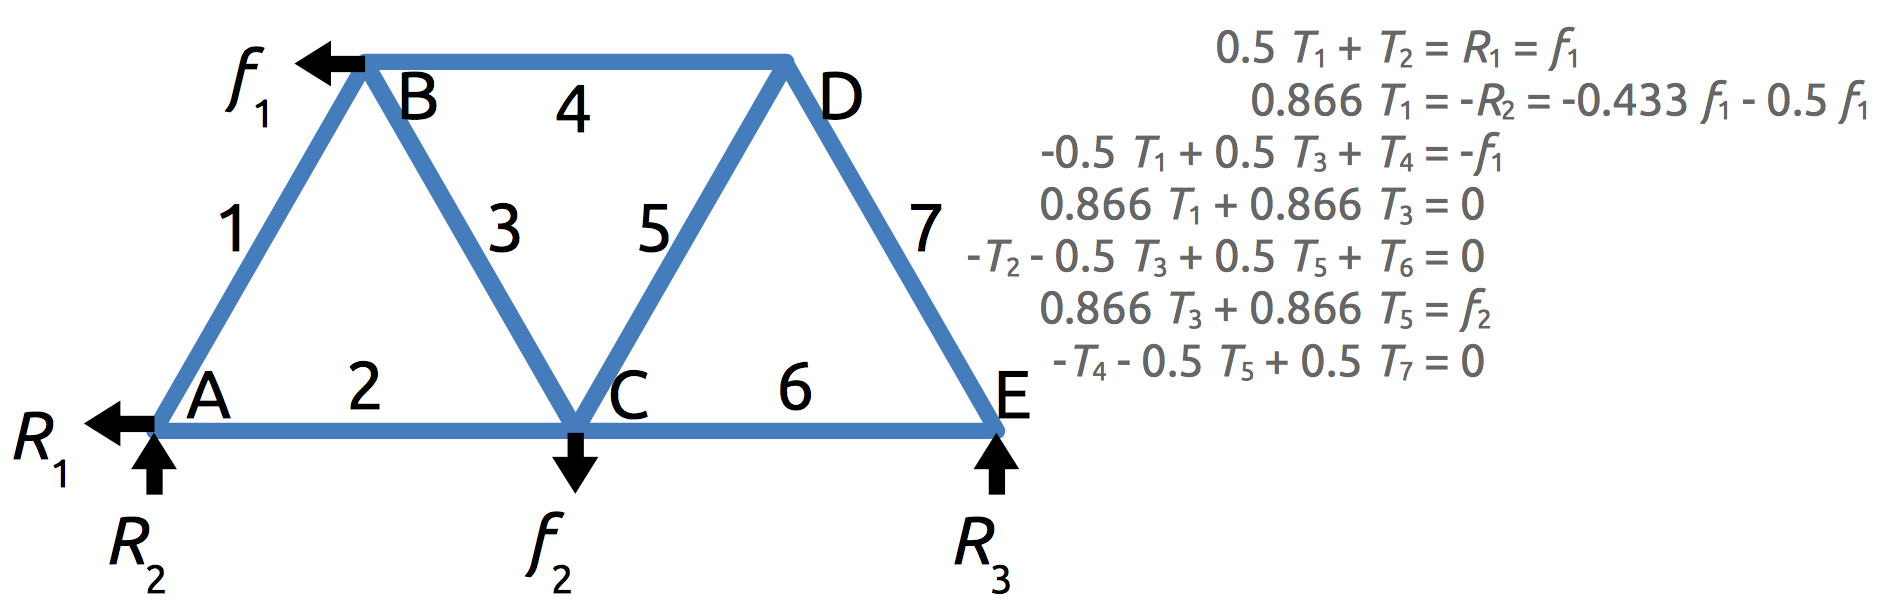
\includegraphics[width=0.8\textwidth]{./truss-graphic.png}
\end{frame}

%%%%%%%%%%%%%%%%%%%%%%%%%%%%%%%%%%%%%%%%%%%%%%%%%%%%%%%%%%%%%%%%%%%%%%%%%%%%%%%
\begin{frame}[fragile]
  \frametitle{Systems of equations}
  %\Enlarge

  $$
\left( \begin{array}{ccccccc}
  0.5 & 1 & 0 & 0 & 0 & 0 & 0 \\
  0.866 & 0 & 0 & 0 & 0 & 0 & 0 \\
  -0.5 & 0 & 0.5 & 0 & 0 & 0 & 0 \\
  0.866 & 0 & 0.866 & 0 & 0 & 0 & 0 \\
  0 & -1 & -0.5 & 0 & 0.5 & 1 & 0 \\
  0 & 0 & 0.866 & 0 & 0.866 & 0 & 0 \\
  0 & 0 & 0 & -1 & -0.5 & 0 & 0.5
\end{array} \right)
\underline{x}
=
\left( \begin{array}{c}
  1000 \\
  -1433 \\
  -1000 \\
  0 \\
  0 \\
  2000 \\
  0
\end{array} \right)
  $$
  $$
\underline{\underline{T}} \underline{x} = \underline{f}
  $$
  %\pause
  \begin{enumerate}
%  \myitem  Use the `New Variable...' interface to define this.
  \end{enumerate}
\end{frame}

%%%%%%%%%%%%%%%%%%%%%%%%%%%%%%%%%%%%%%%%%%%%%%%%%%%%%%%%%%%%%%%%%%%%%%%%%%%%%%%
\begin{frame}[fragile]
  \frametitle{Solution finding}
  \Enlarge

  \begin{enumerate}
  \myitem  An effective way to solve equations is to set the left- and right-hand sides to equal each other.
  \end{enumerate}
  $$
\exp\left( -\sin^2 bx \right)
=
2 - x^2
  $$
  %\pause
  \begin{enumerate}
  \myitem  OR, subtract so they go to zero:
  \end{enumerate}
  $$
\exp\left( -\sin^2 bx \right) - 2 + x^2
=
0
  $$
  %\pause
  \begin{Verbatim}
function [ rhs ] = lhs( x )
    b = 1.0;
    rhs = exp(-sin(b.*x).^2) - 2 + x.^2;
end
fplot( @lhs,[ -10 10 ] );
fzero( @lhs,0 );
  \end{Verbatim}
\end{frame}

%%%%%%%%%%%%%%%%%%%%%%%%%%%%%%%%%%%%%%%%%%%%%%%%%%%%%%%%%%%%%%%%%%%%%%%%%%%%%%%
\begin{frame}[fragile]
  \frametitle{Solution finding}
  \Enlarge

  \begin{enumerate}
  \myitem  Polynomial \texttt{roots} are also easy to find:
  \end{enumerate}
  $$
2 x^3 + 3 x^2 - 4 x - 5 = 0
  $$
  %\pause
  \begin{Verbatim}
roots( [ 2 3 -4 -5 ] )
  \end{Verbatim}
\end{frame}

%%%%%%%%%%%%%%%%%%%%%%%%%%%%%%%%%%%%%%%%%%%%%%%%%%%%%%%%%%%%%%%%%%%%%%%%%%%%%%%%
\begin{frame}[fragile]
  \frametitle{Question}
  \Enlarge

  \begin{Verbatim}
A = [ 5 4 1- 2 2 ];
B = [ 5 4 1 -2 2 ];
  \end{Verbatim}

Are \texttt{A} and \texttt{B} equal in value?

  \begin{enumerate}[label=\Alph*]
    \item  Yes
    \item  No
  \end{enumerate}
\end{frame}

%%%%%%%%%%%%%%%%%%%%%%%%%%%%%%%%%%%%%%%%%%%%%%%%%%%%%%%%%%%%%%%%%%%%%%%%%%%%%%%%
\begin{frame}[fragile]
  \frametitle{Question}
  \Enlarge

  \begin{Verbatim}
A = [ 5 4 1- 2 2 ];
B = [ 5 4 1 -2 2 ];
  \end{Verbatim}

Are \texttt{A} and \texttt{B} equal in value?

  \begin{enumerate}[label=\Alph*]
    \item  Yes
    \item  No  \correctstar
  \end{enumerate}
\end{frame}

% - PDE toolbox example?
% - find factorial using function browser

\end{document}
